\subsection{Results}
The data from the UMBmark test were used to plot three robot paths.
The points at which the robot stopped to turn were marked on the floor,
and were used as reference points.
The laser range scanner and odometry readings were sent to a PC,
and were processed using the aforementioned algorithms.
A problem occured in the test: some laser range scanner readings were lost,
possibly due to partial incompatibility between the PC's OS and the serial communication library used.

%The UMB-test was conducted as follows:
%
%\begin{enumerate}
%\item The robots start position of the robots wheels where marked on the floor.
%\item The robot then drives 1m forward, using the given library, and then holds a break. If it returned to this point for the 20th time, it stops. \label{item:driveForward}
%\item During the robots pause, the position of the robots wheels were, again, marked on the floor.
%\item The robot then turns $90^{\circ}$ to the left and continues then from point \ref{item:driveForward}. 
%\end{enumerate}

%During the course of this test data from the encoders and 2D laser scanner were collected for off-line processing. 
%Furthermore the actual position of the robot was measured.
%Afterwards the start, end and intermediate positions of the robot were measured.

%The data was then used to find the robots position given the two datasets. 
%Because of faults first discovered later, there were inconsistencies in the data collection.
%The datasets where hence reduced to include only the beginning of the dataset till just before the point where the corruption was too great to be used for positioning the robot on the map.

However, the line-based localisation algorithm was able to match the features correctly for several
rounds, and the results have been plotted in figure \ref{fig:comparisonOfEncoderVSScanner}.

\begin{figure}[H]
\centering
\makebox[\textwidth][c]{
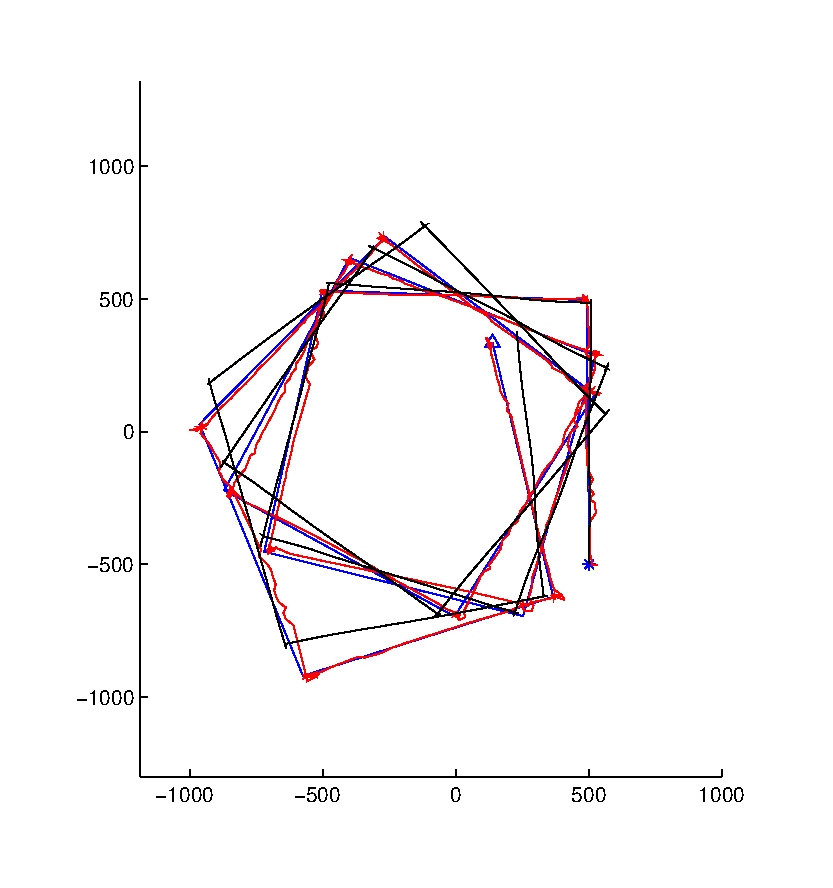
\includegraphics[width = 15cm,trim= 1cm 1cm 1cm 1cm ,clip=true]{graphics/comparison_encoderVSscanner}}
\caption[Comparison of the two localization methods.]{Comparison of the two localization methods.
The blue line connects the reference points where the robot paused to turn,
$*$ is the starting position and $\Delta$ is the ending position.
The red line represents the 2D laser range scanner localisation and the black line represents the odometry readings.}
\label{fig:comparisonOfEncoderVSScanner}
\end{figure}

It is easily seen that the line-based localisation algorithm is better than odometry alone.
The line-based localisation seems to move in distorted lines, and this indicates the actual movement
better than the reference lines; the reference lines are just straight lines drawn between the reference points.

%\todo[inline,author=Mikael]{Vi mangler resultater for orientering :-)}

The results were expected, as the odometry method accumulates error over time, and the line-based method does not.

The deviations of the two models for calculating the position of the robot are seen in figure \ref{fig:deviationOfEncoderVSScanner}.
The figure shows the deviation of the robot at the reference points, where the robot paused.

\begin{figure}[H]
\centering
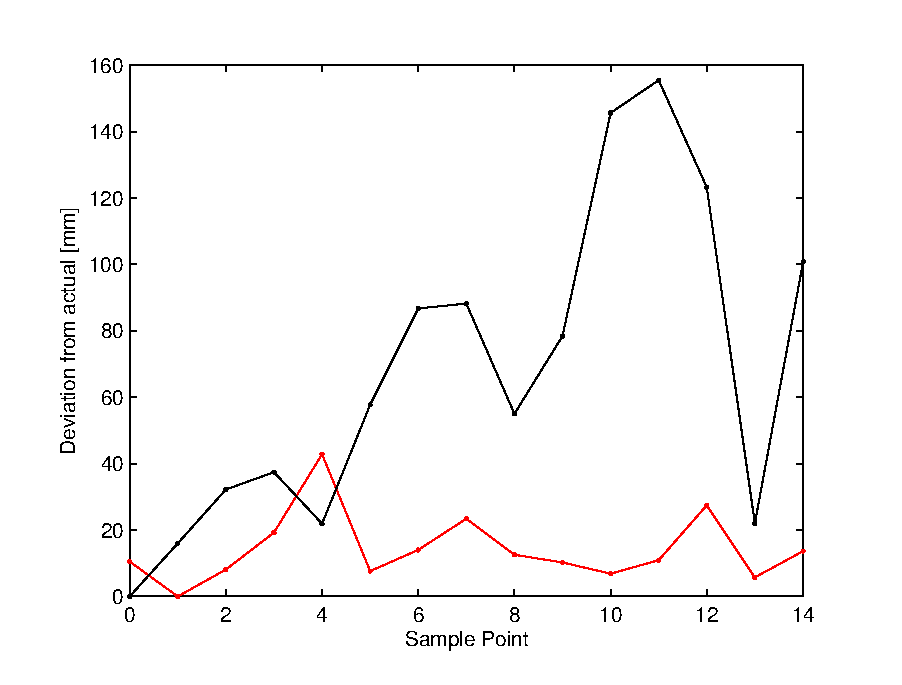
\includegraphics[width = 13cm]{graphics/deviation_encoderVSscanner}
\caption[Deviation in position of the two localization methods.]{Deviation in position of the two localization methods. The red line represents the laser range scanner localisation, and the black line represents the odometry readings.}
\label{fig:deviationOfEncoderVSScanner}
\end{figure}

From figure \ref{fig:deviationOfEncoderVSScanner} it can be seen that the error accumulates over time
when using only odometry to measure the position.
The data from the laser range scanner, however, are used to calculate the position considerably better,
with a much more steady deviation, than the odometry readings.

When plotting the absolute deviation of the robots angle at the previous used points figure \ref{fig:deviationOfEncoderVSScannerAngle} is obtained.


\begin{figure}[H]
\centering
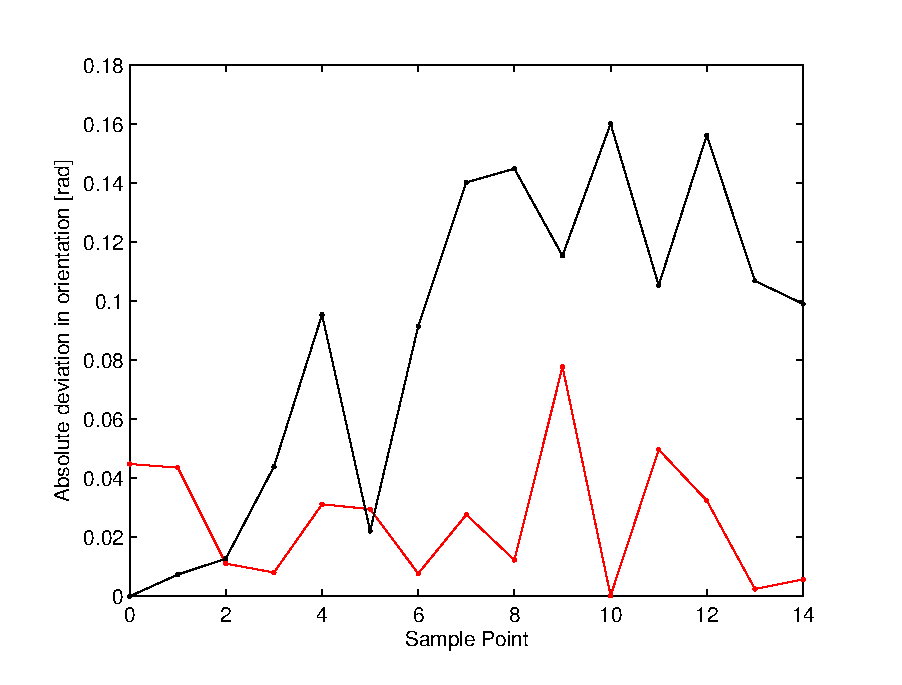
\includegraphics[width = 13cm]{graphics/deviation_angle_encoderVSscanner}
\caption[Deviation in orientation of the two localization methods.]{Deviation in orientation of the two localization methods. The red line represents the laser range scanner localisation, and the black line represents the odometry readings.}
\label{fig:deviationOfEncoderVSScannerAngle}
\end{figure}

It can from figure \ref{fig:deviationOfEncoderVSScannerAngle} be seen that the deviation in orientation is, like for the position, accumulating over time. 
The odometry is for short distances and few turns better or equal that of the average laser scanner readings. This advantage does, however, cease when the robot reaches its fourth turn and onwards it is considerably higher.

It can hence be concluded that the laser scanner is considerably better when driving for longer time and only one method of localisation has to be used.
The combination of using both the laser scanner and odometry together is, however, recommendable.
Odometry alone is not suitable to stand alone, but they can be used efficiently in combination to achieve accurate localization of a robot on a map.
It should still be noted that odometry can be used to accurately decide the robots position and angle when travelling short distances.
